\chapter{Why the Thermodynamic Cost of Erasing History Matters}

I want readers to understand something that many academic circles are only beginning to explore: erasing history is not just a moral or cultural loss — it is a calculable act of destruction. There is a \textit{cost} associated with it. And that cost is not only societal or ideological. It is physical. It is thermodynamic.

Drawing from Shannon entropy, Huffman coding, and Rolf Landauer’s thermodynamic theory of information, every attempt to delete a fact — to erase even a single \textit{bit} of truth — carries an irreversible energy cost.

\begin{figure}[h]
\centering
\includegraphics[width=0.8\textwidth]{assets/entropy_erasure_plot.png}
\caption{Minimum energy cost of erasing 1 bit of information, per Landauer's Principle.}
\end{figure}

\[
E_{\text{min}} = kT \ln(2)
\]

The deletion of truth is not clean. It is not free. It is entropy-in-action, and it demands our resistance — with precision, data, and moral clarity.

\begin{figure}[h]
\centering
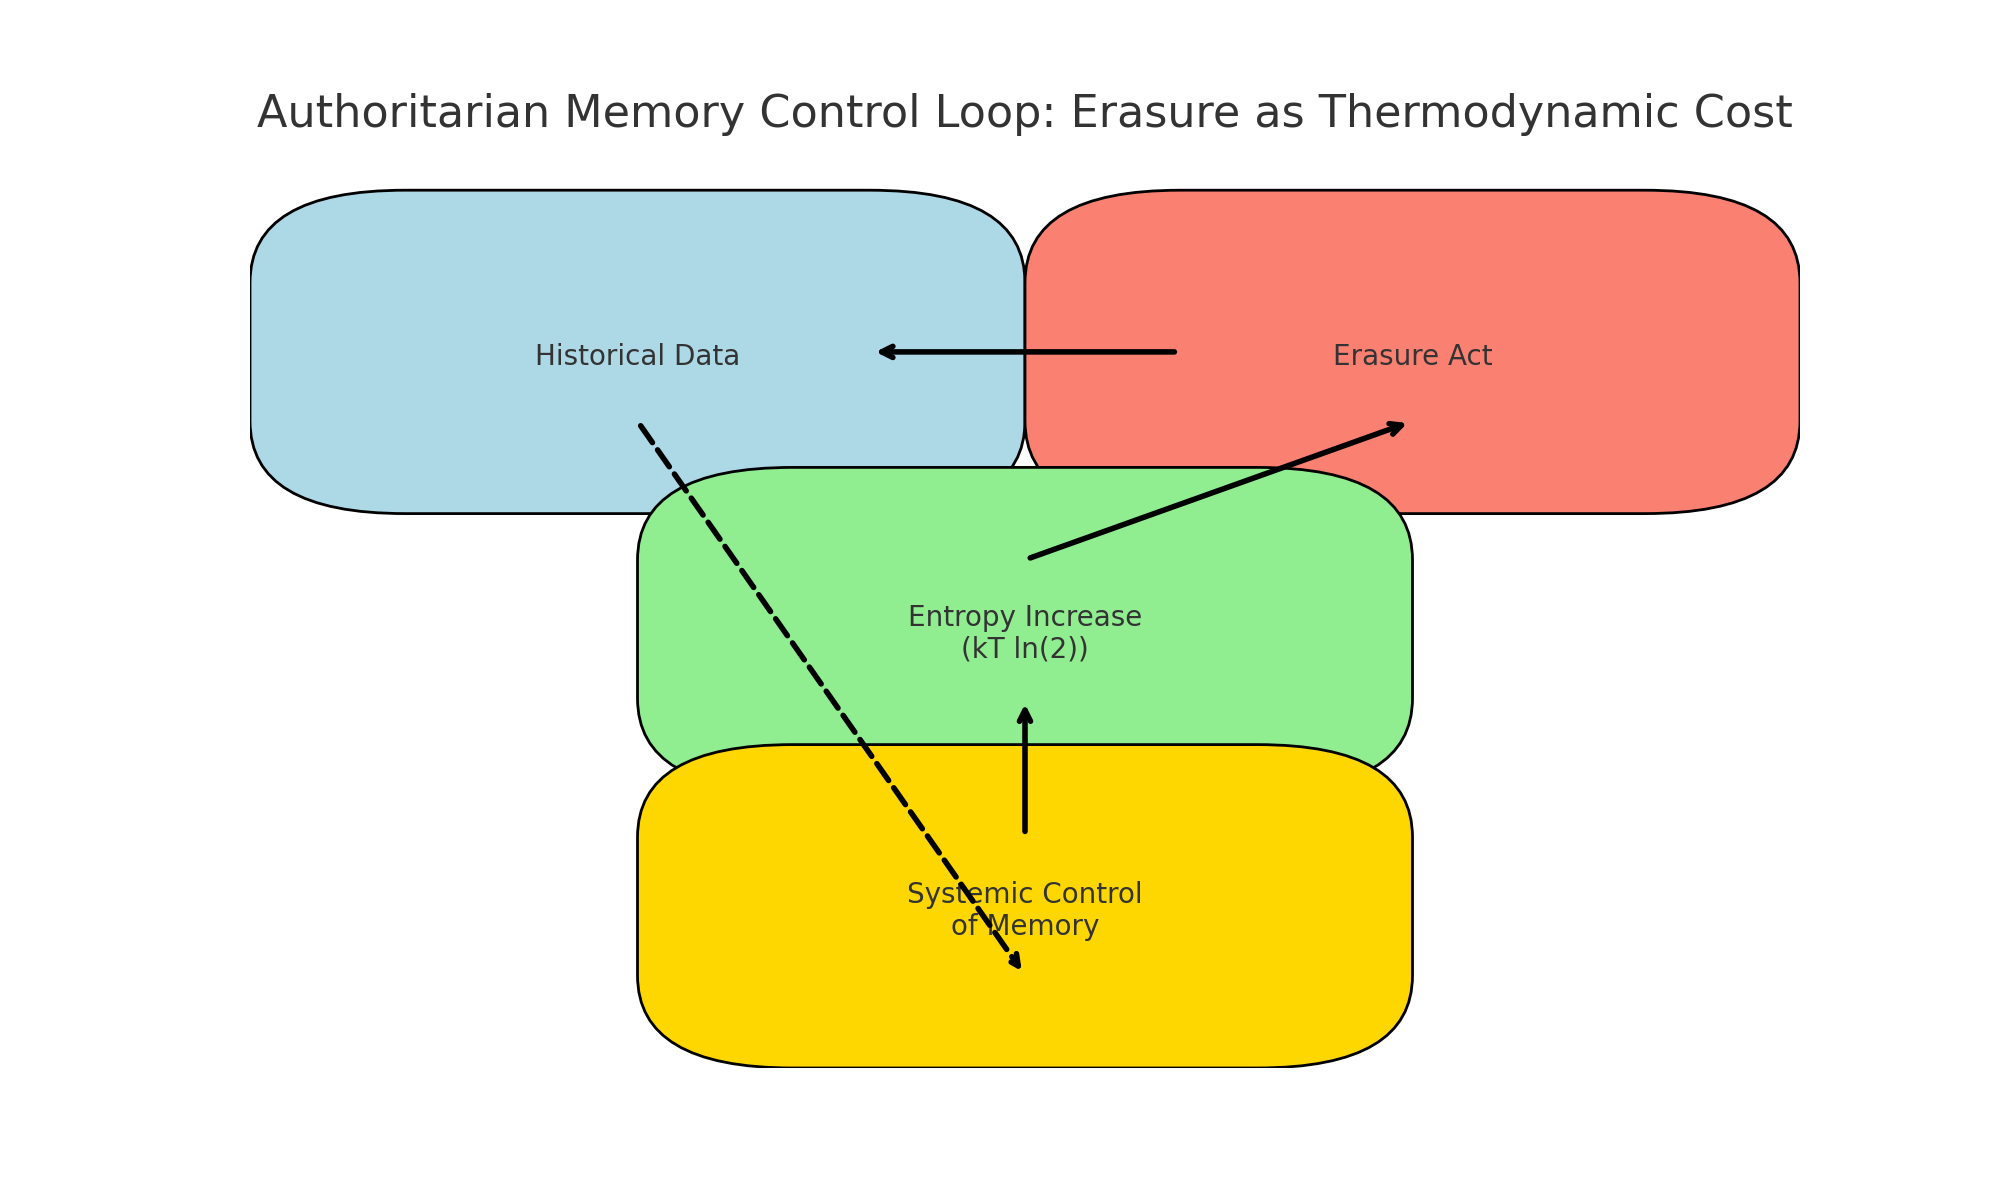
\includegraphics[width=0.8\textwidth]{assets/entropy_erasure_feedback.png}
\caption{Authoritarian memory control loop: erasure of historical data as a thermodynamic act.}
\end{figure}
